This chapter contains theoretical information about the paper's domain, deep learning,
and the principal model used, autoencoders.
Of course, before starting looking in its domain,
we should start with the basics, namely, machine learning.
\section{What is Machine Learning?}

Machine learning is one of many subfields of artificial intelligence,
the science of getting the computer to learn from experience
without being explicitly programmed to do so,
improving their ability to think, plan, decide, etc. \cite{whatIsML}.\par
Algorithms in this area are different in their approach, the type of data they input and output,
and the type of problem they are learning to
solve, but, despite all differences, they are based on the same idea that there are some
generic algorithms that can discover patterns,
without having to write code; instead, they build their own logic on the data fed to them.
% \vspace{0.5cm}

% @HERE
\section{Machine Learning Styles}
When studying machine learning, one can identify a plethora of algorithms,
each unique in its approach and purpose, but all of them can be classified
based on the learning style. Therefore, there can be grouped into four main categories:
\begin{itemize}
    \item \textbf{Supervised Learning}
    \item \textbf{Unsupervised Learning}
    \item \textbf{Semi-supervised Learning}
    \item \textbf{Reinforcement Learning}
\end{itemize}
\vspace{0.5cm}

% @HERE
\subsection{Supervised Learning}
In supervised learning, given a set of example input-output pairs,
the job of the algorithms is to approximate a function that maps from input to output \cite{amai}.
It is called supervised learning because human experts act as the teacher,
where they serve the computer with training data containing the input and
also provide the correct output, from which the computer should be able to observe patterns.
As seen depicted in the Figure\emph{~\ref{fig:supervised}}, the algorithm should be able
to predict the output given new inputs,
based on  the function that it approximates \cite{typesMLMedium}.

\begin{figure}[h]
    \centering
    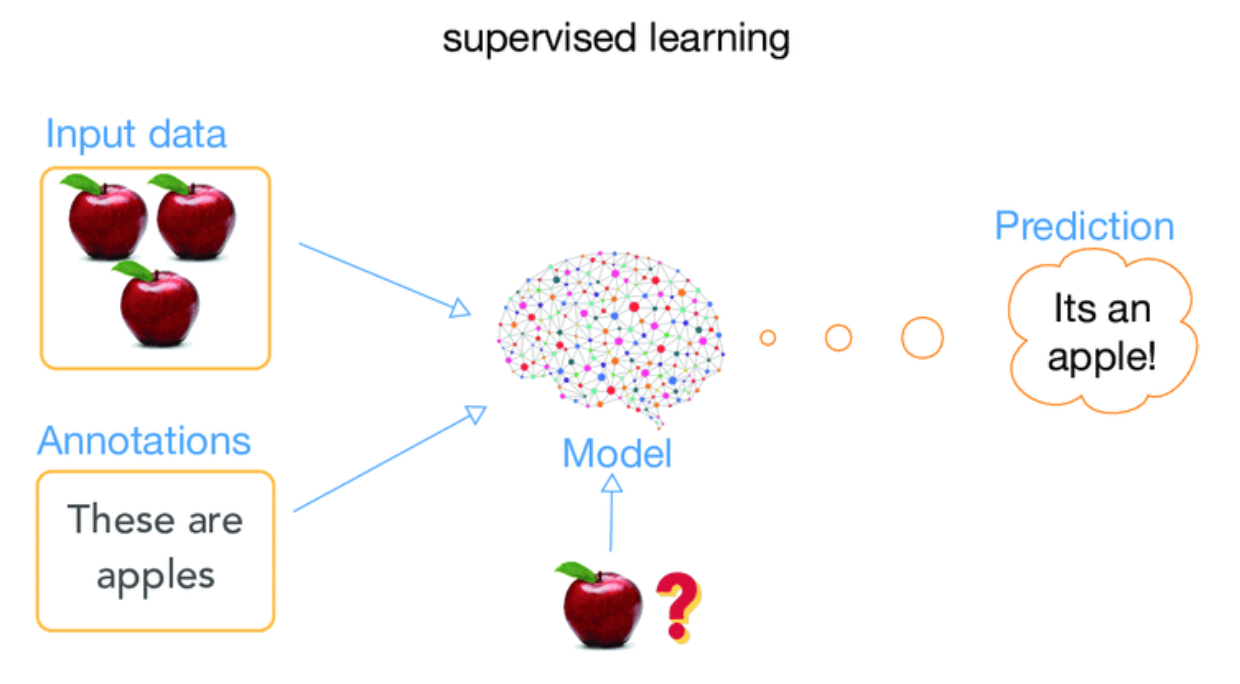
\includegraphics[width=1\textwidth]{supervised_learning}
    \caption{\emph{Supervised algorithm predicting new output data given new input  \cite{typesML}}}
    \label{fig:supervised}
\end{figure}

Furthermore, supervised machine learning algorithms can also
be grouped based on the type of problem they intend to solve.
Having said that, there are classification and regression algorithms.

% @HERE Classification
Classification algorithms solve problems in which the input data has
been labelled in different classes or categories,
meaning that the goal  is to predict discrete values
such as $\{0, 1\}$, $\{2, 4, 6, 8\dots\}$, $\{cat, dog\}$, $\{spam, normal\}$, etc.

% @HERE Regression
Regression algorithms, on the other hand, solve problems in which the output variable
is a real value, meaning that the goal is to predict continuous values based on the
input data, such as predicting house prices based on their size and location.

\begin{figure}[h]
    \centering
    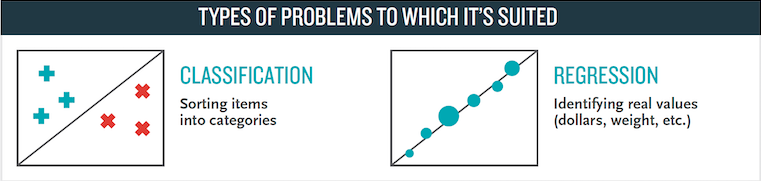
\includegraphics[width=1\textwidth]{regression_classification}
    \caption{\emph{Classification(left) and Regression(right) visualization  \cite{bigDataR}}}
    \label{fig:regression_classification}
\end{figure}


\subsection{Unsupervised Learning}
WIP







\subsection{Semi-supervised Learning}
WIP
\subsection{Reinforcement Learning}
WIP

\section{ANN's and how they work}
One of the main types of machine learning algorithms that are vastly used is
artificial neural networks or ANNs.
They are structured as weighted graphs, modelled after the
human brain where each node represents a neuron and each
edge represents the synapses of the neural network.
The weight of each edge determines how powerful the synapse is.
The neurons are distributed in groups named layers.
Neurons can form synapses only with neurons from other layers.
\vspace{0.5cm}

As you can see in \emph{\ref{fig:ann_structure}} there are three types of layers in an artificial neural network:
\begin{itemize}[]
    \item{ Input layer
          \begin{adjustwidth}{1cm}{}
              This layer of a neural network is the very beginning of the ANN’s workflow, bringing the initial data into the system for
              further processing by subsequent layers of artificial neurons \cite{inputLayer}.
          \end{adjustwidth}
          }
    \item{ Hidden layer
          \begin{adjustwidth}{1cm}{}
              Any layer between the output and the input layer is considered to be a hidden layer.
              The number of neurons they contain and also their number can vary.
              Their role is to take in a set of weighted inputs and produce an output through an activation function \cite{hiddenlayer}.
          \end{adjustwidth}
          }
    \item{ Output layer
          \begin{adjustwidth}{1cm}{}
              This layer of a neural network is the last layer of neurons that produces given outputs for the program.
              They usually are made much like any other artificial neuron, but they may be observed in a different way,
              the output layer coalesces and concretely produces the end result \cite{outputLayer}.
          \end{adjustwidth}
          }
\end{itemize}
\begin{figure}[h]
    \centering
    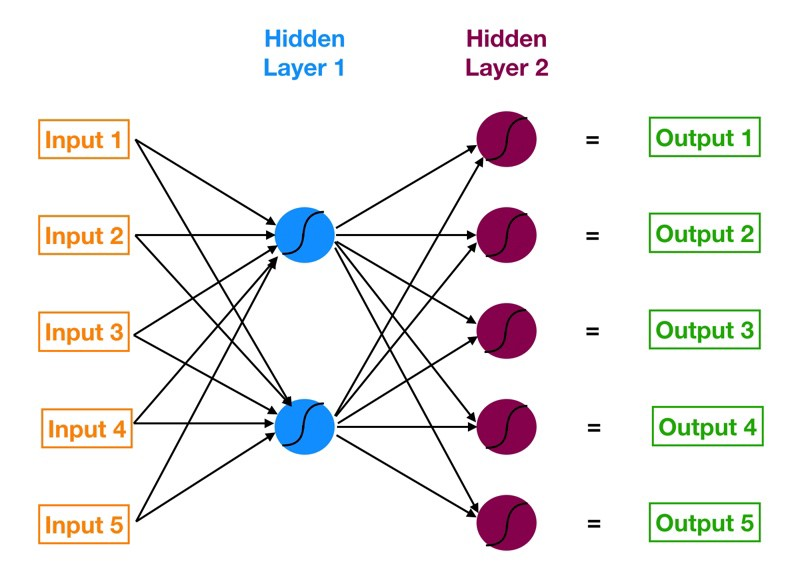
\includegraphics[width=1\textwidth]{ann_structure}
    \caption{\emph{Neural network with one hidden layer \cite{understandingANN}}}
    \label{fig:ann_structure}
\end{figure}


\section{What is Deep Learning?}

Deep learning is a subfield of machine learning that contains a collection of ANNs that are known for
their capability on learning unsupervised from data that is unstructured or unlabeled,
also known as deep neural learning or deep neural network.

\vspace{0.5cm}
A second classification we can make on ANNs is based on the relationships between their nodes.
Then, neural networks can be recurrent or feedforward;
the first one does not have any loops in its graph and can be organized in layers.
A deep neural network is a feedforward ANN with many hidden layers.
\vspace{5cm}

A visual representation of the aforementioned is the Figure\emph{~\ref{fig:deep_vs_normal}} wherein we could see
the differences between a simple feedforward ANN with one hidden layer(left) and a deep neural network with three
hidden layers
\begin{figure}[h]
    \centering
    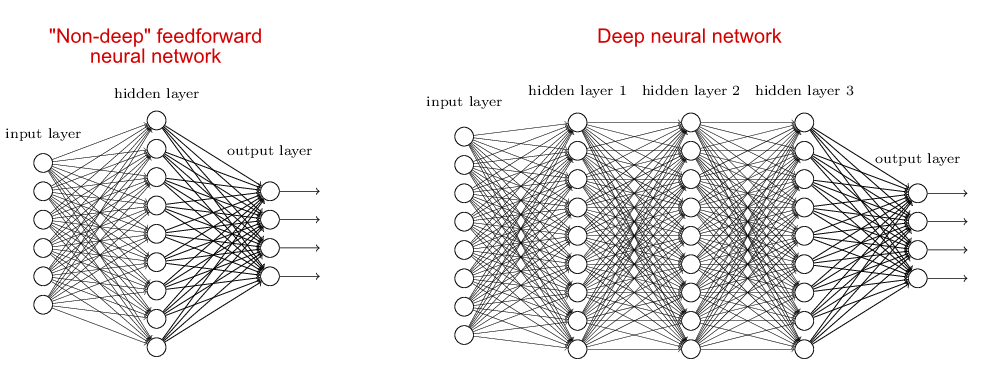
\includegraphics[width=1\textwidth]{deep_vs_normal_ann}
    \caption{\emph{Difference between a Non-deep ANN(left) and a deep ANN(right) \cite{deepLearningBook}}}
    \label{fig:deep_vs_normal}
\end{figure}

